\chapter{Projekt}
\section{Przypadki użycia}
\section{Prototyp interfejsu}
\begin{minipage}{\textwidth}
    \begin{figure}[H]
        \centering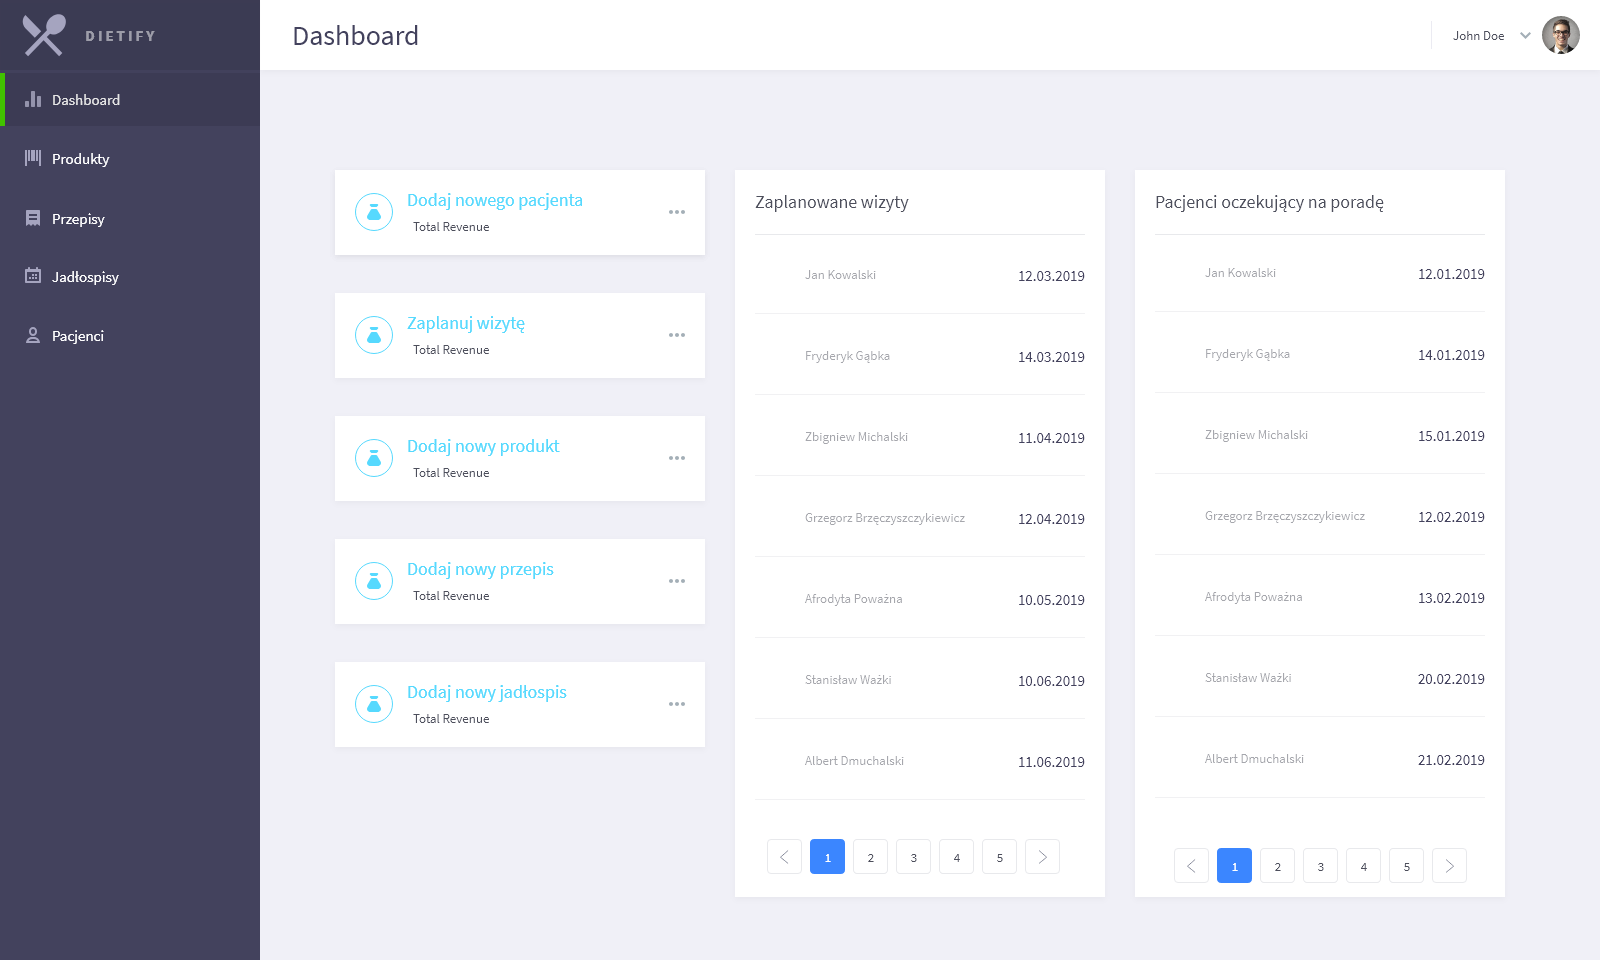
\includegraphics[width=0.9\textwidth]{img/mockups/mockup1.png}
        \caption{Mockup1 (opr.wł).}\label{rysunek:mockup1}
    \end{figure}
\end{minipage}

\begin{minipage}{\textwidth}
    \begin{figure}[H]
        \centering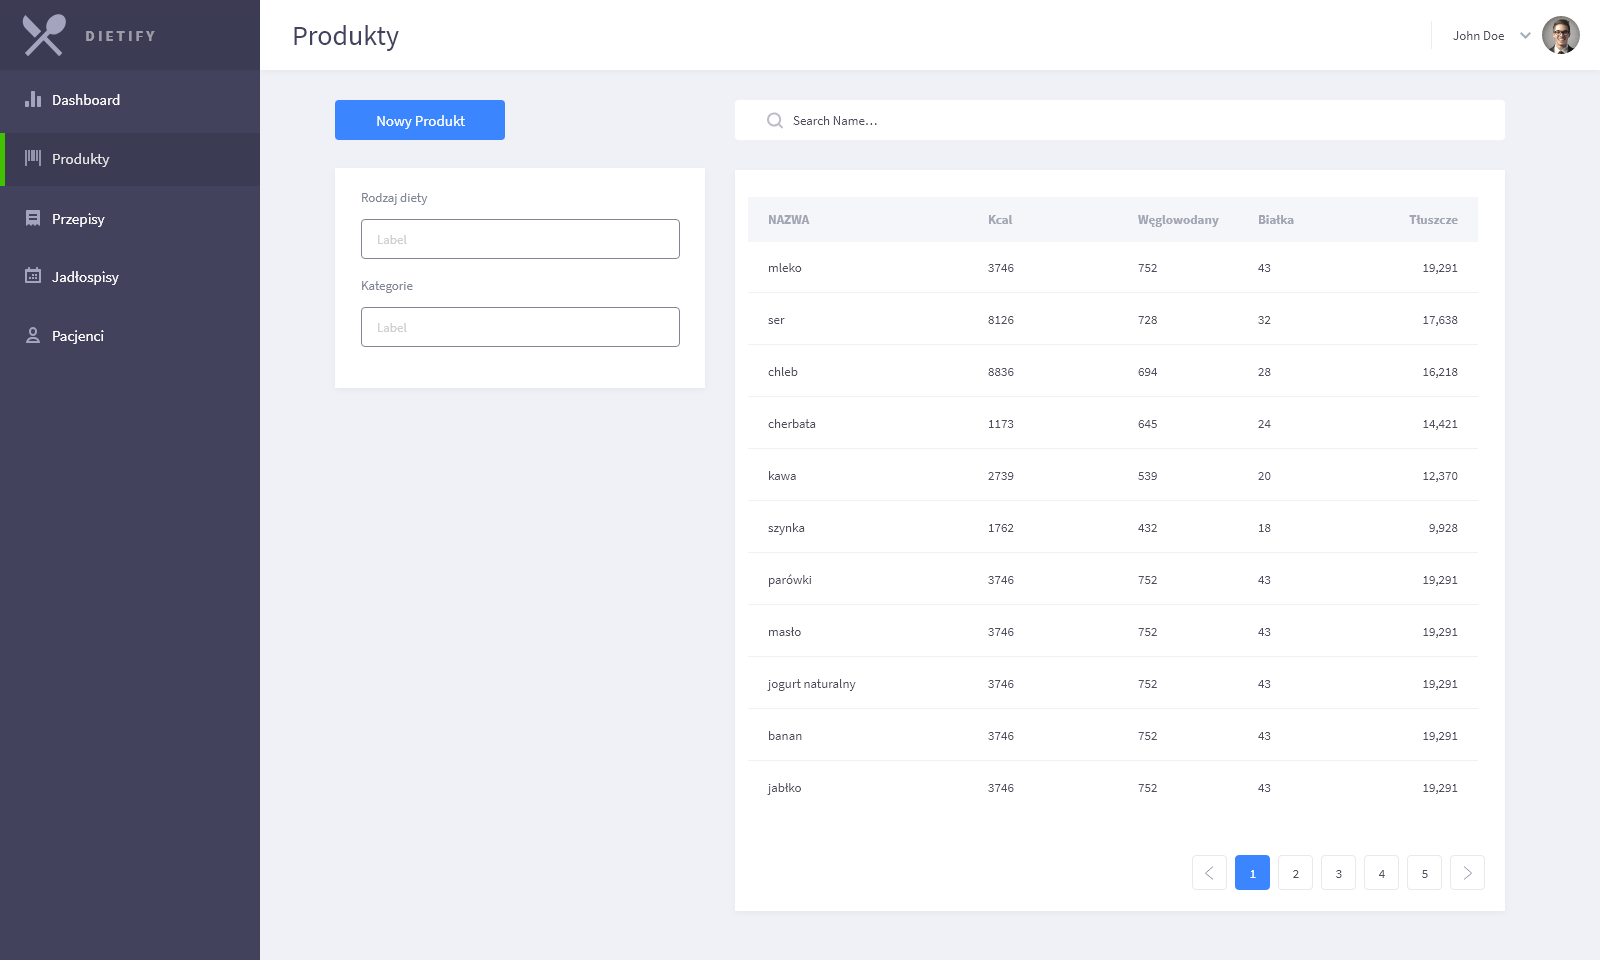
\includegraphics[width=0.9\textwidth]{img/mockups/mockup2.png}
        \caption{Mockup2 (opr.wł).}\label{rysunek:mockup2}
    \end{figure}
\end{minipage}

\begin{minipage}{\textwidth}
    \begin{figure}[H]
        \centering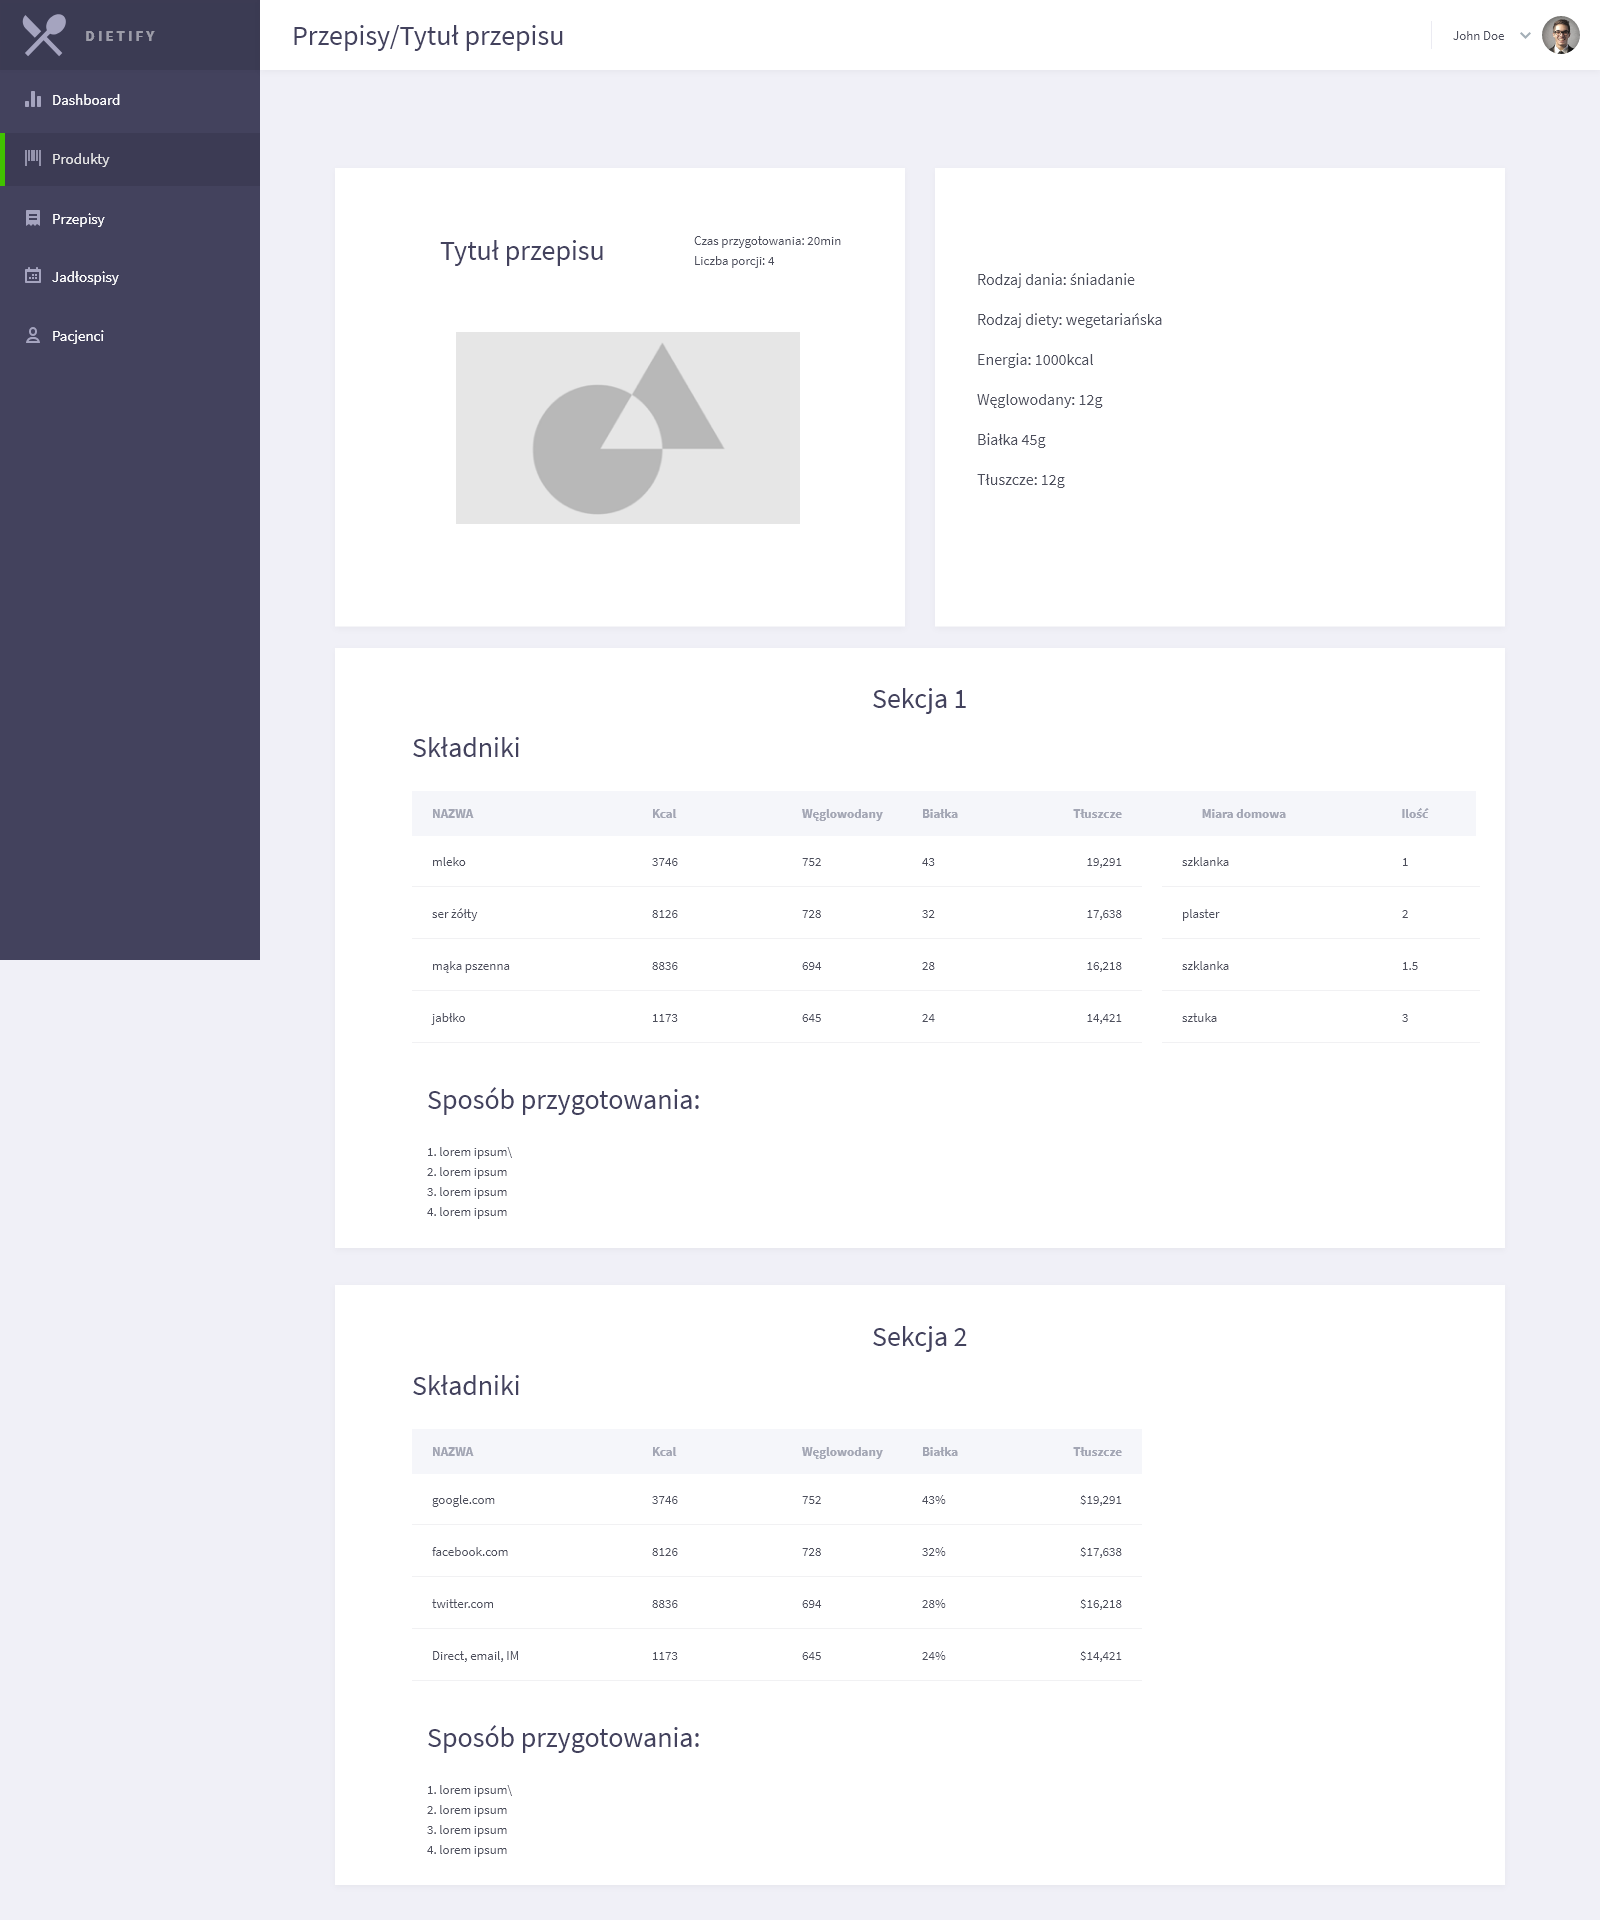
\includegraphics[width=0.9\textwidth]{img/mockups/mockup3.png}
        \caption{Mockup3 (opr.wł).}\label{rysunek:mockup3}
    \end{figure}
\end{minipage}

\begin{minipage}{\textwidth}
    \begin{figure}[H]
        \centering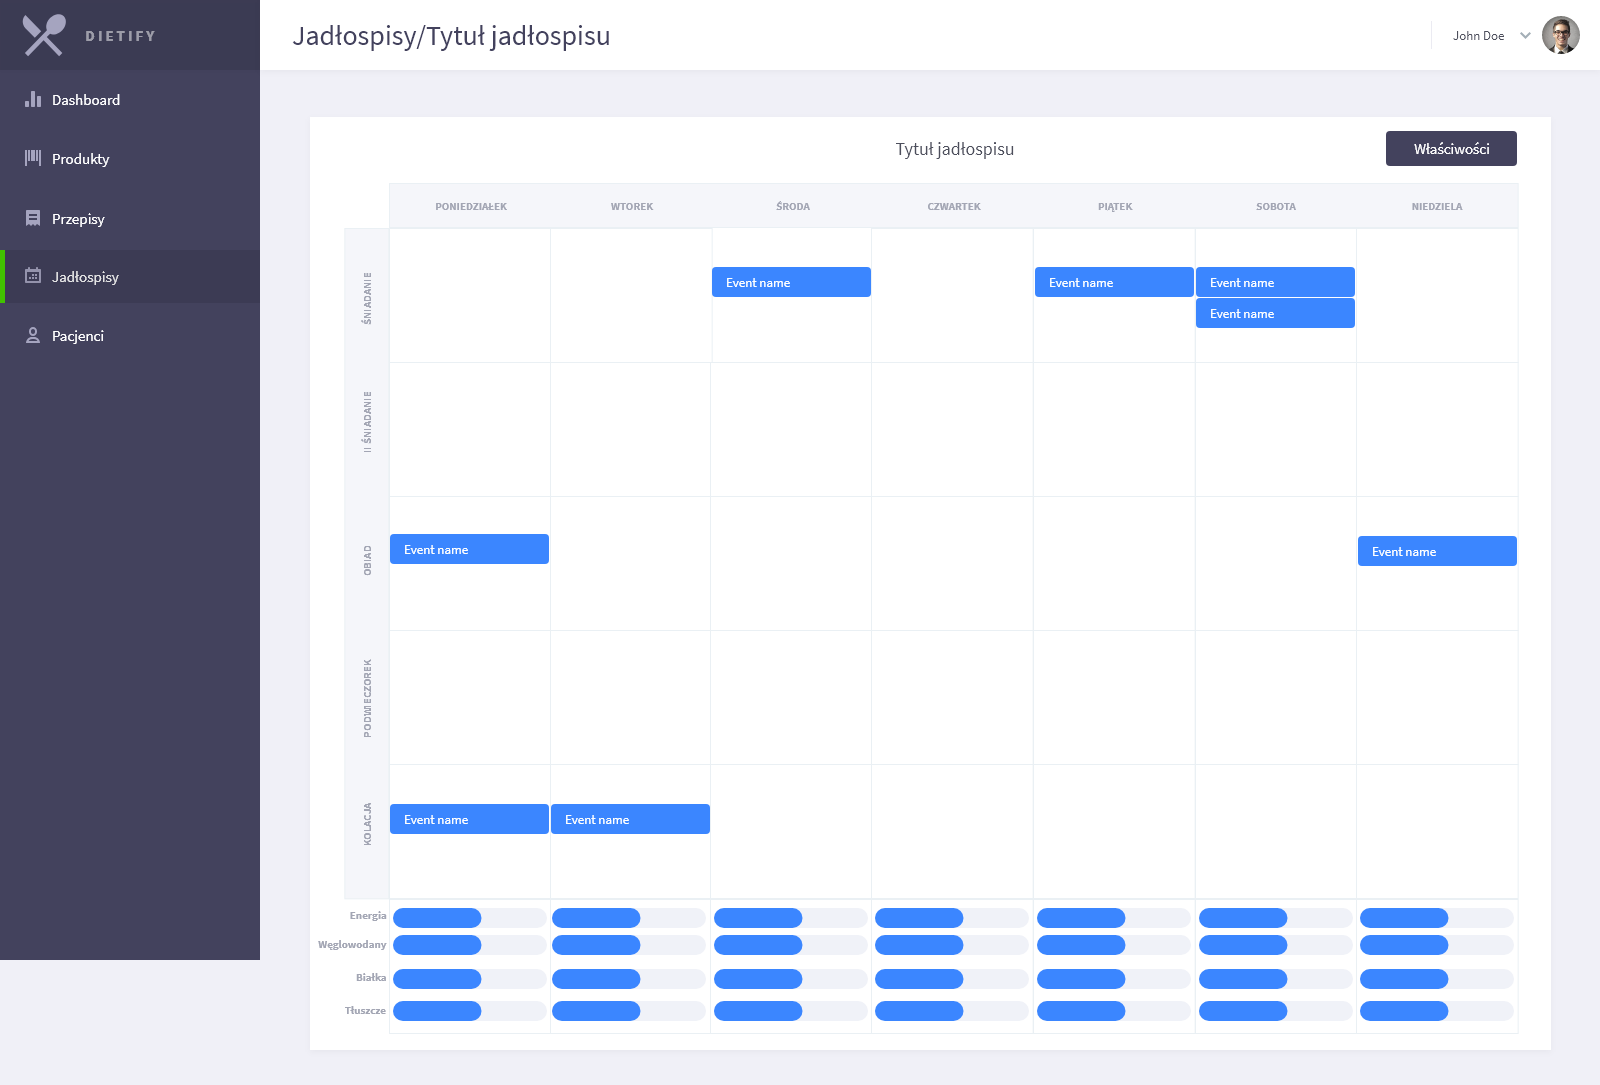
\includegraphics[width=0.9\textwidth]{img/mockups/mockup4.png}
        \caption{Mockup4 (opr.wł).}\label{rysunek:mockup4}
    \end{figure}
\end{minipage}

\begin{minipage}{\textwidth}
    \begin{figure}[H]
        \centering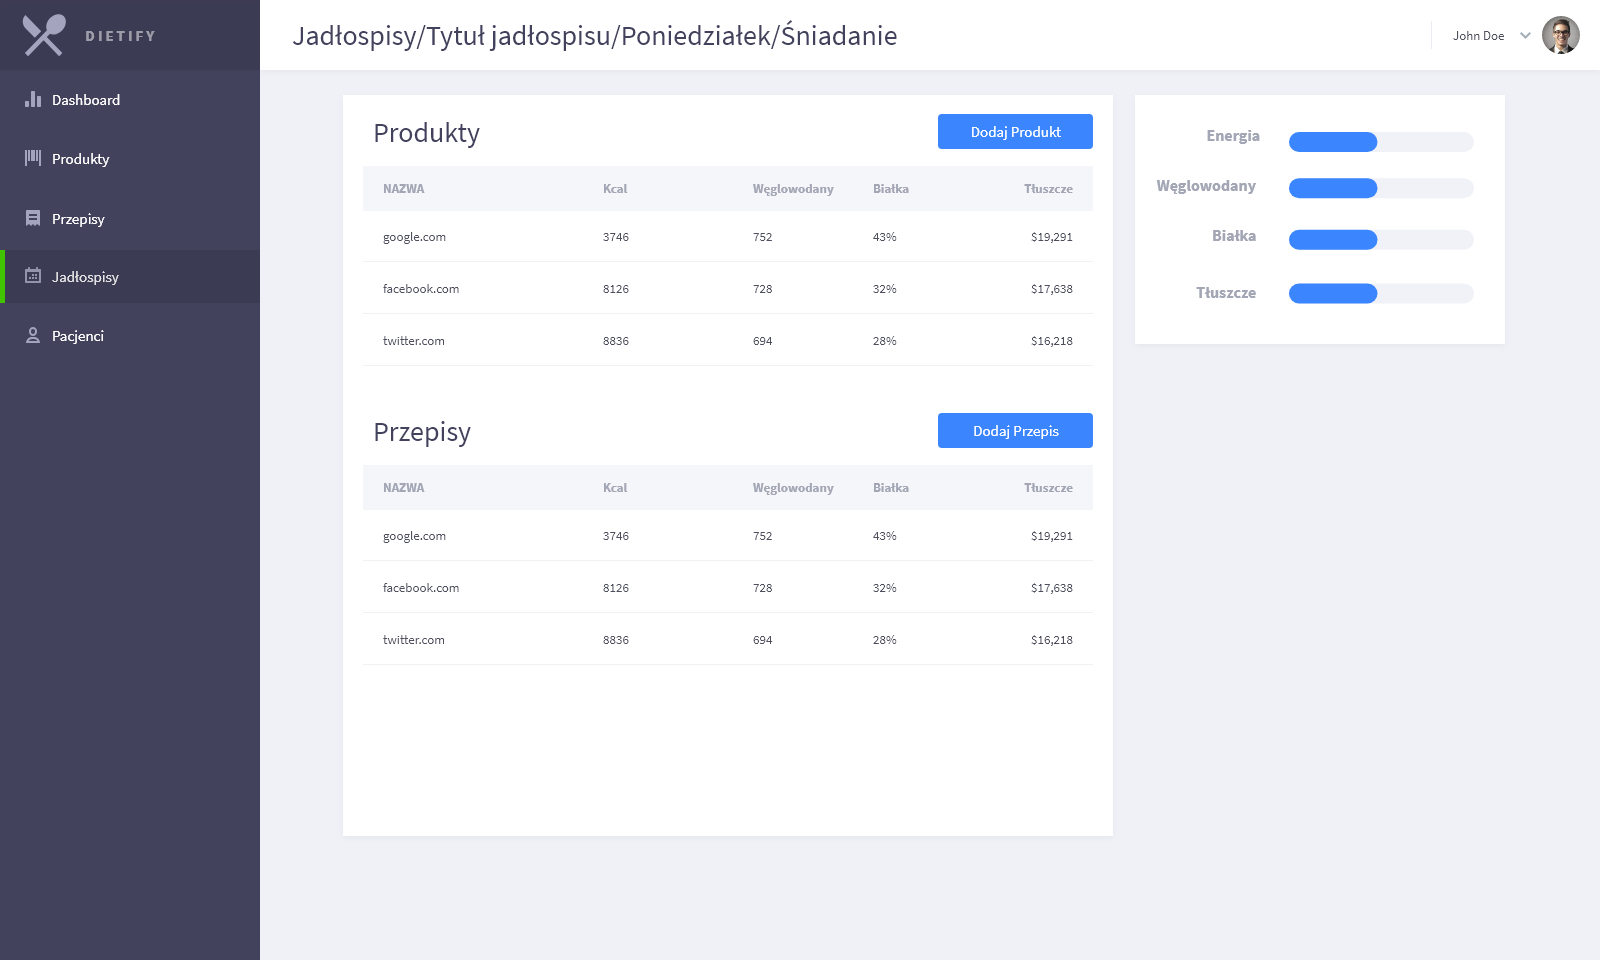
\includegraphics[width=0.9\textwidth]{img/mockups/mockup5.png}
        \caption{Mockup5 (opr.wł).}\label{rysunek:mockup5}
    \end{figure}
\end{minipage}

\begin{minipage}{\textwidth}
    \begin{figure}[H]
        \centering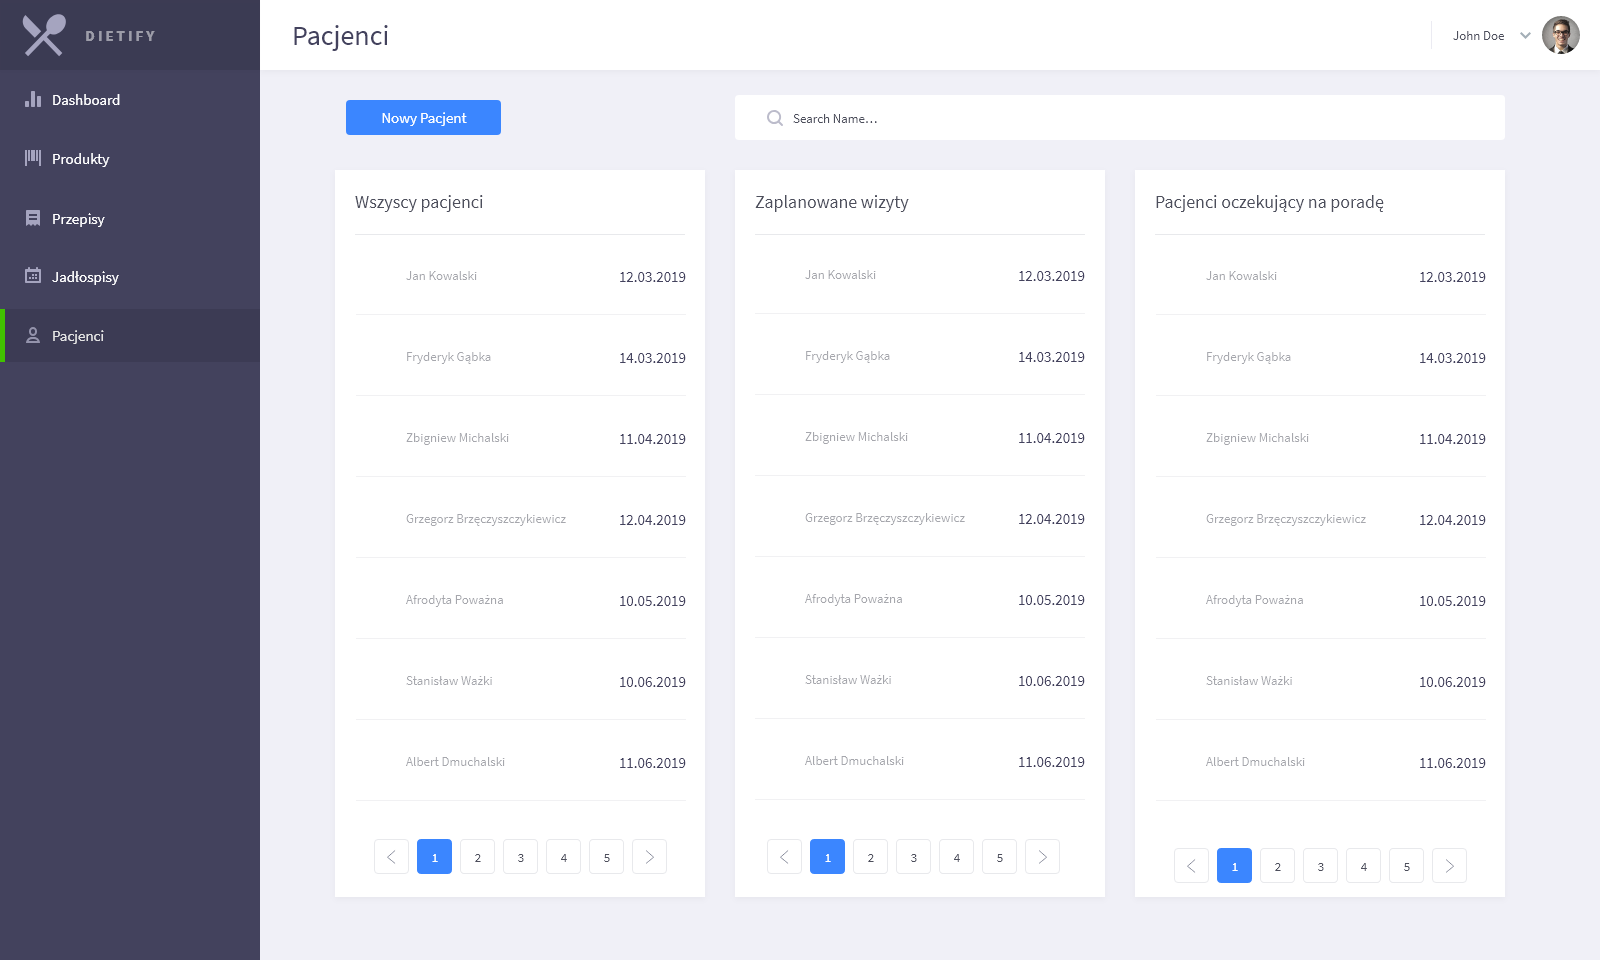
\includegraphics[width=0.9\textwidth]{img/mockups/mockup6.png}
        \caption{Mockup6 (opr.wł).}\label{rysunek:mockup6}
    \end{figure}
\end{minipage}

\begin{minipage}{\textwidth}
    \begin{figure}[H]
        \centering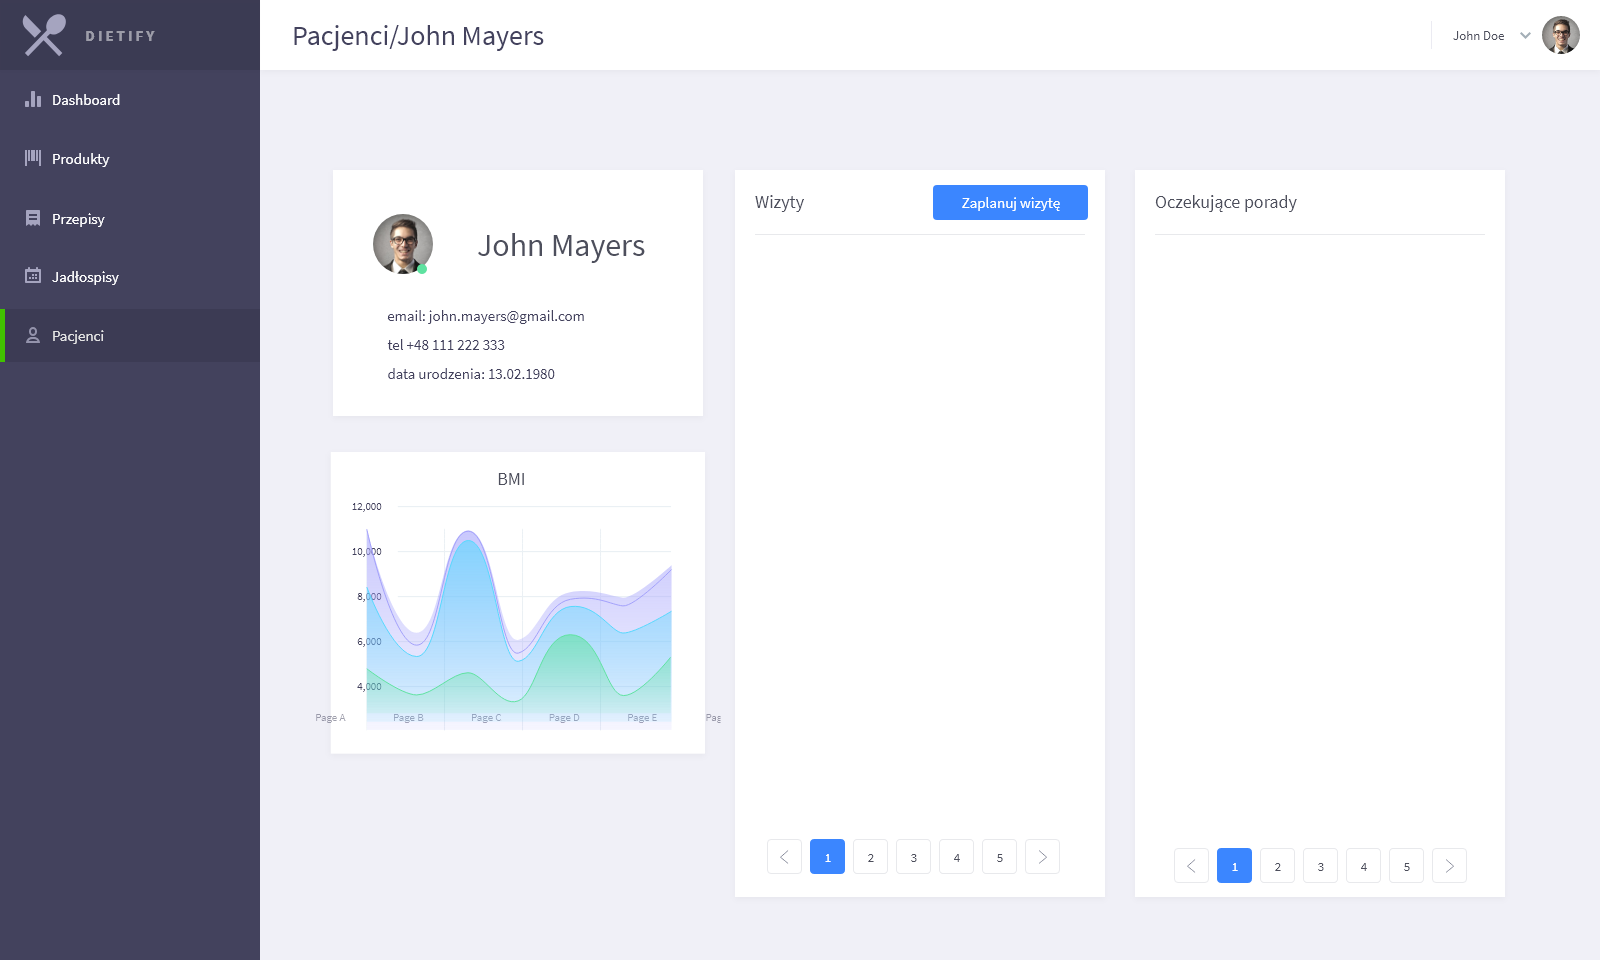
\includegraphics[width=0.9\textwidth]{img/mockups/mockup7.png}
        \caption{Mockup7 (opr.wł).}\label{rysunek:mockup7}
    \end{figure}
\end{minipage}

\begin{minipage}{\textwidth}
    \begin{figure}[H]
        \centering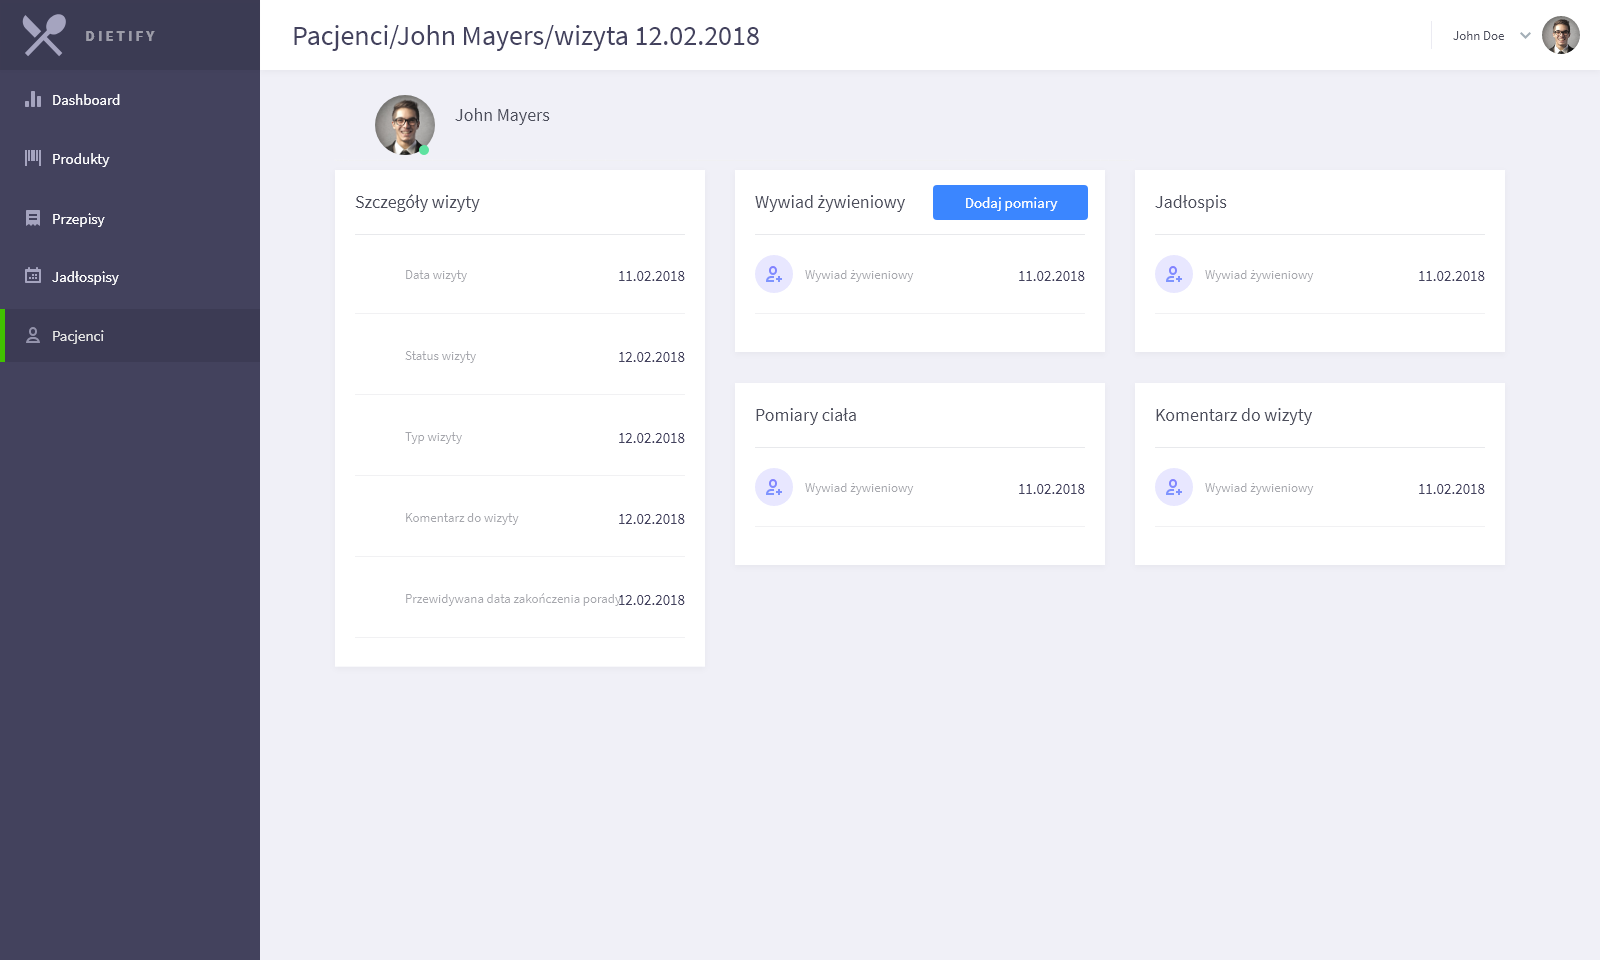
\includegraphics[width=0.9\textwidth]{img/mockups/mockup8.png}
        \caption{Mockup8 (opr.wł).}\label{rysunek:mockup8}
    \end{figure}
\end{minipage}

\begin{minipage}{\textwidth}
    \begin{figure}[H]
        \centering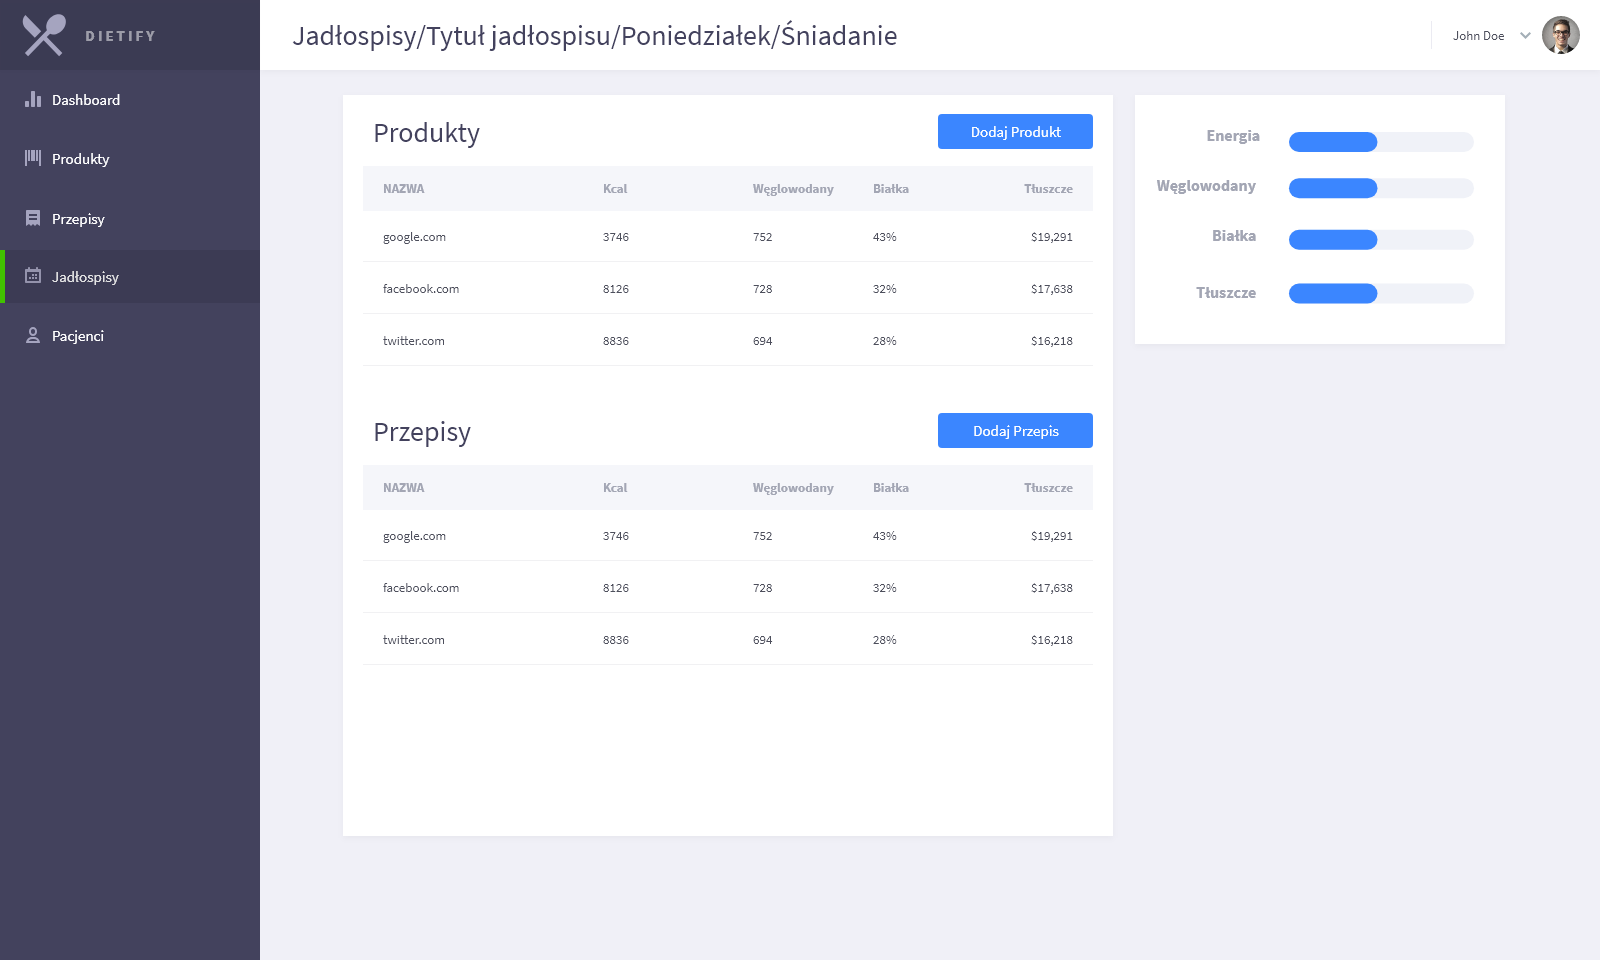
\includegraphics[width=0.9\textwidth]{img/mockups/mockup9.png}
        \caption{Mockup9 (opr.wł).}\label{rysunek:mockup9}
    \end{figure}
\end{minipage}

\begin{minipage}{\textwidth}
    \begin{figure}[H]
        \centering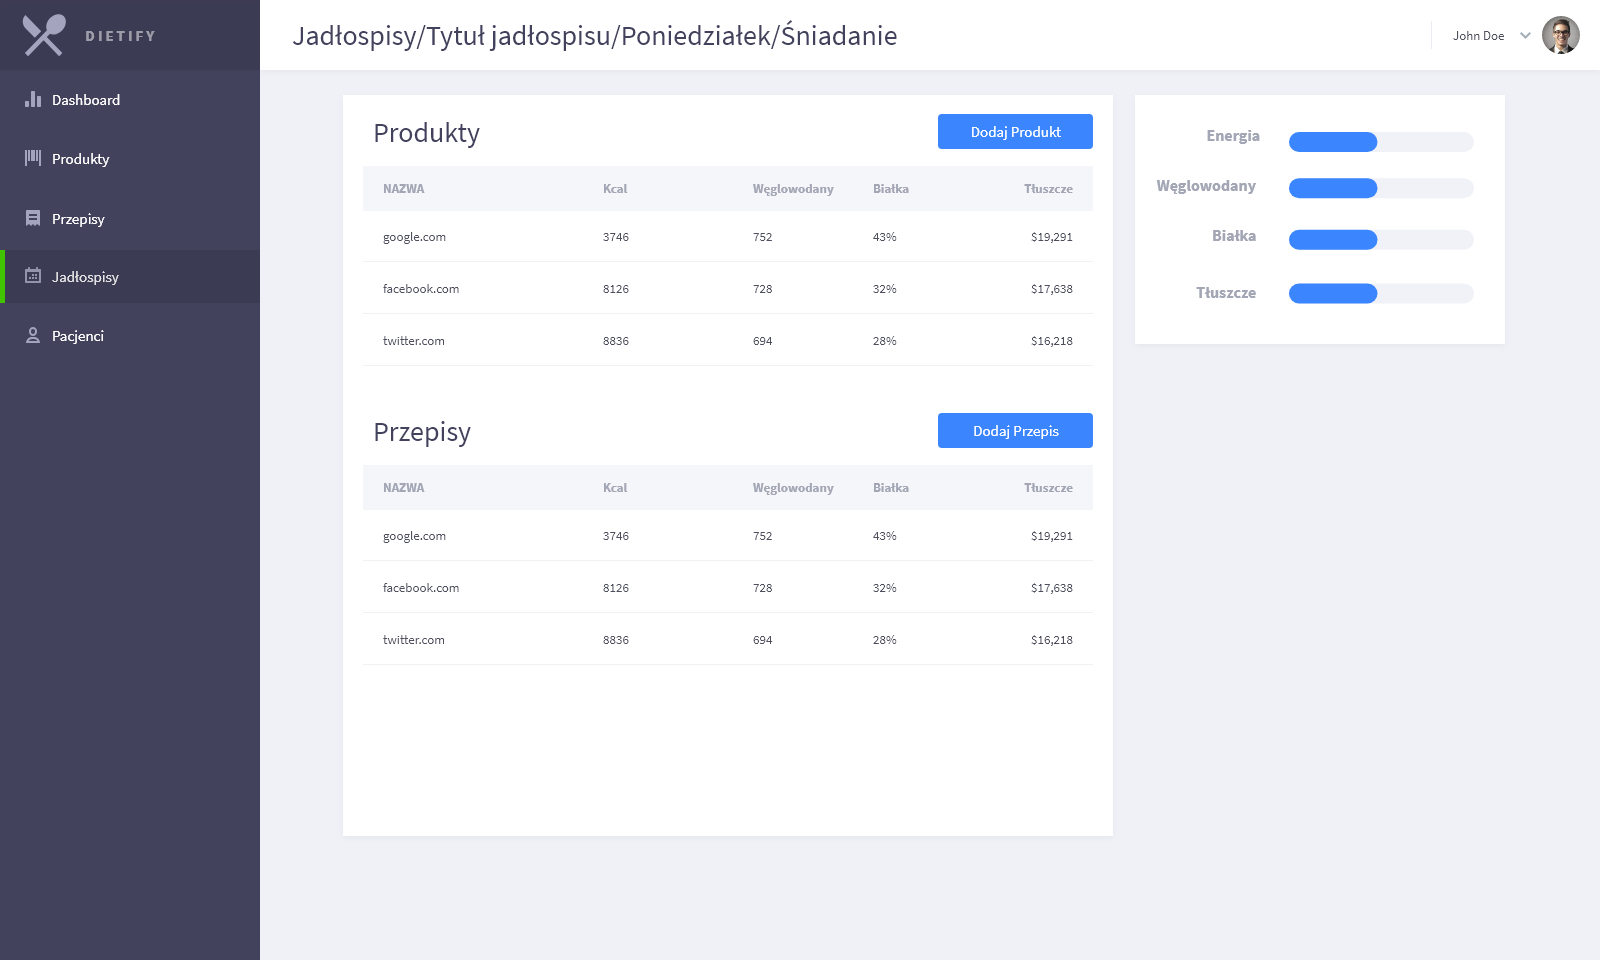
\includegraphics[width=0.9\textwidth]{img/mockups/mockup10.png}
        \caption{Mockup10 (opr.wł).}\label{rysunek:mockup10}
    \end{figure}
\end{minipage}

\begin{minipage}{\textwidth}
    \begin{figure}[H]
        \centering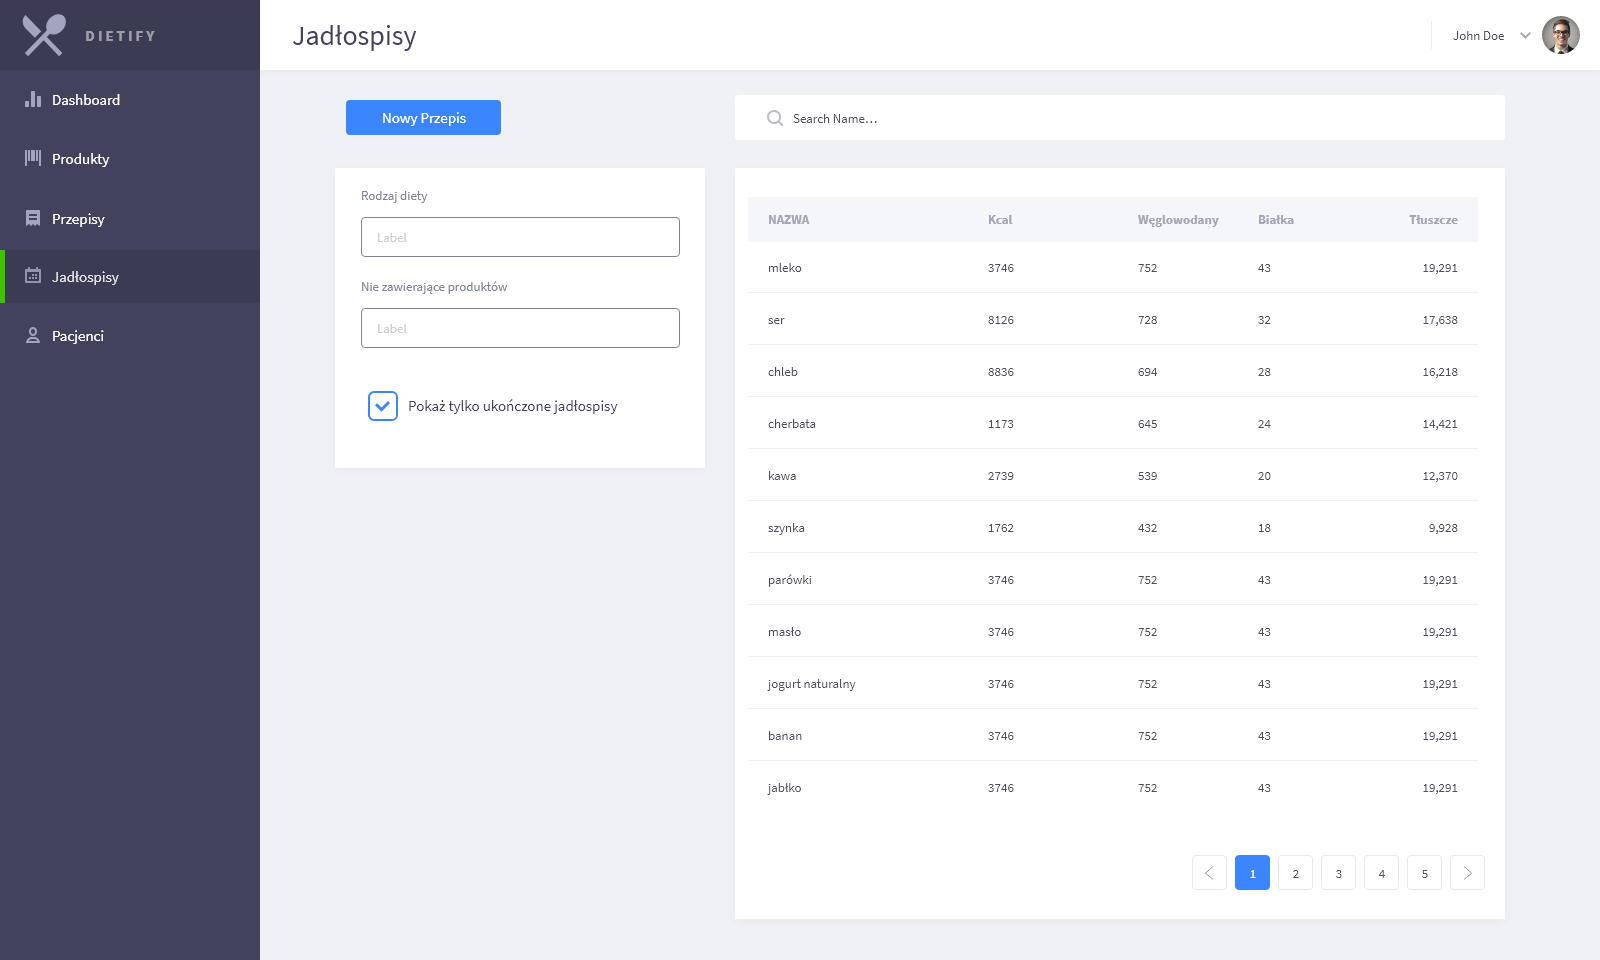
\includegraphics[width=0.9\textwidth]{img/mockups/mockup11.png}
        \caption{Mockup11 (opr.wł).}\label{rysunek:mockup11}
    \end{figure}
\end{minipage}

\begin{minipage}{\textwidth}
    \begin{figure}[H]
        \centering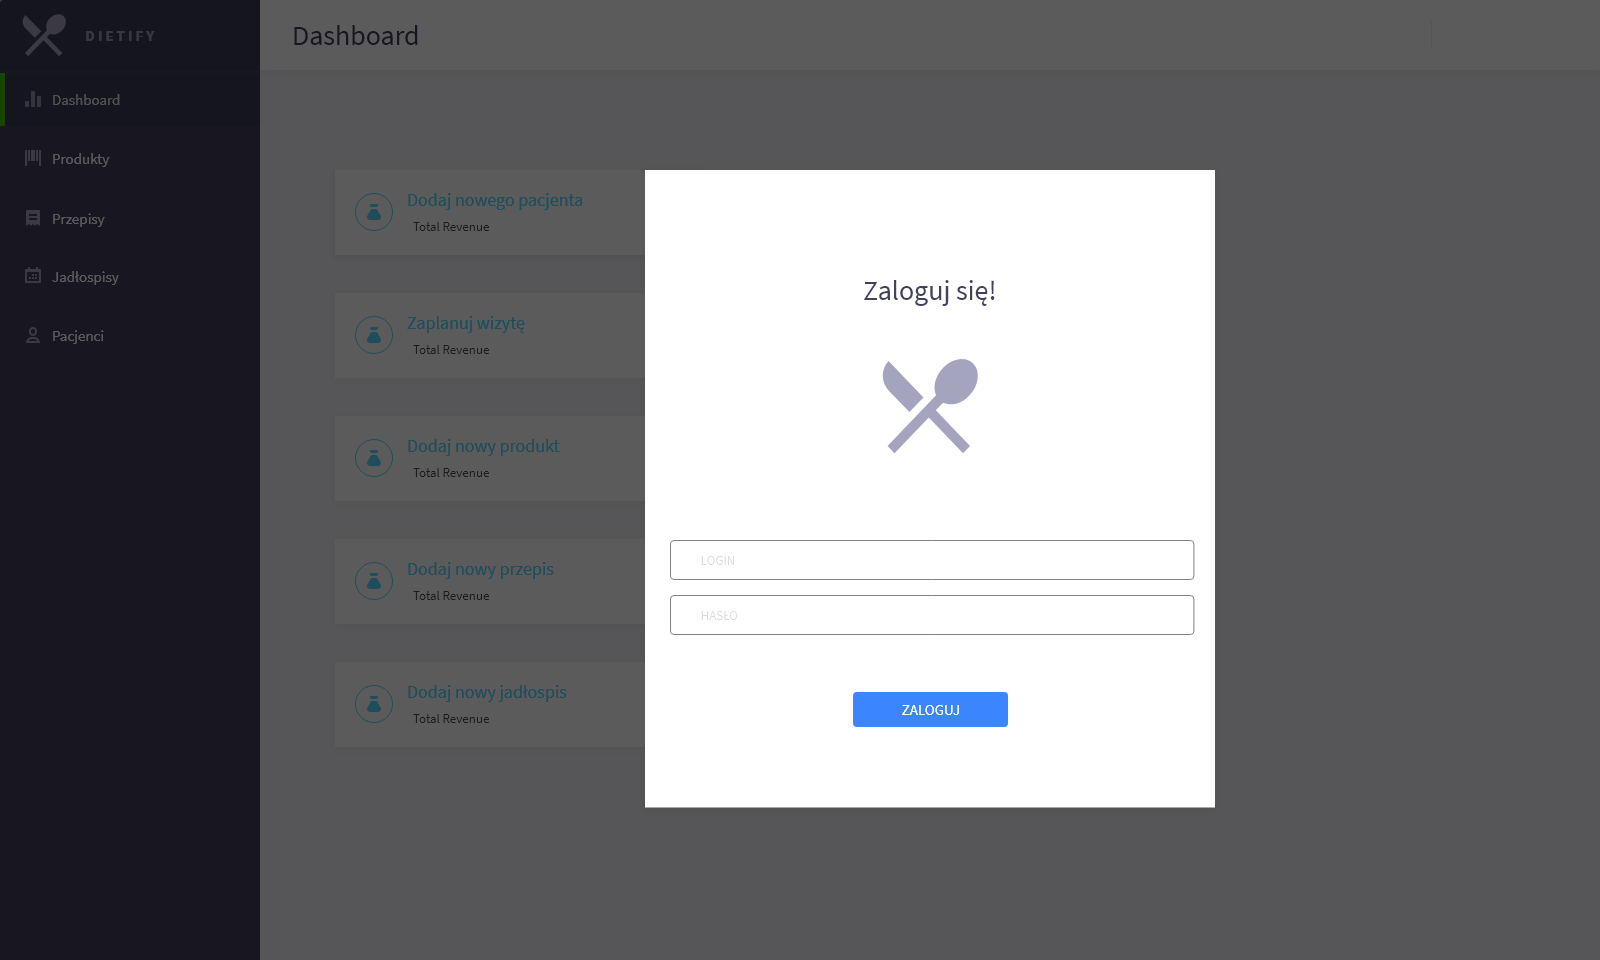
\includegraphics[width=0.9\textwidth]{img/mockups/mockup12.png}
        \caption{Mockup12 (opr.wł).}\label{rysunek:mockup12}
    \end{figure}
\end{minipage}

\begin{minipage}{\textwidth}
    \begin{figure}[H]
        \centering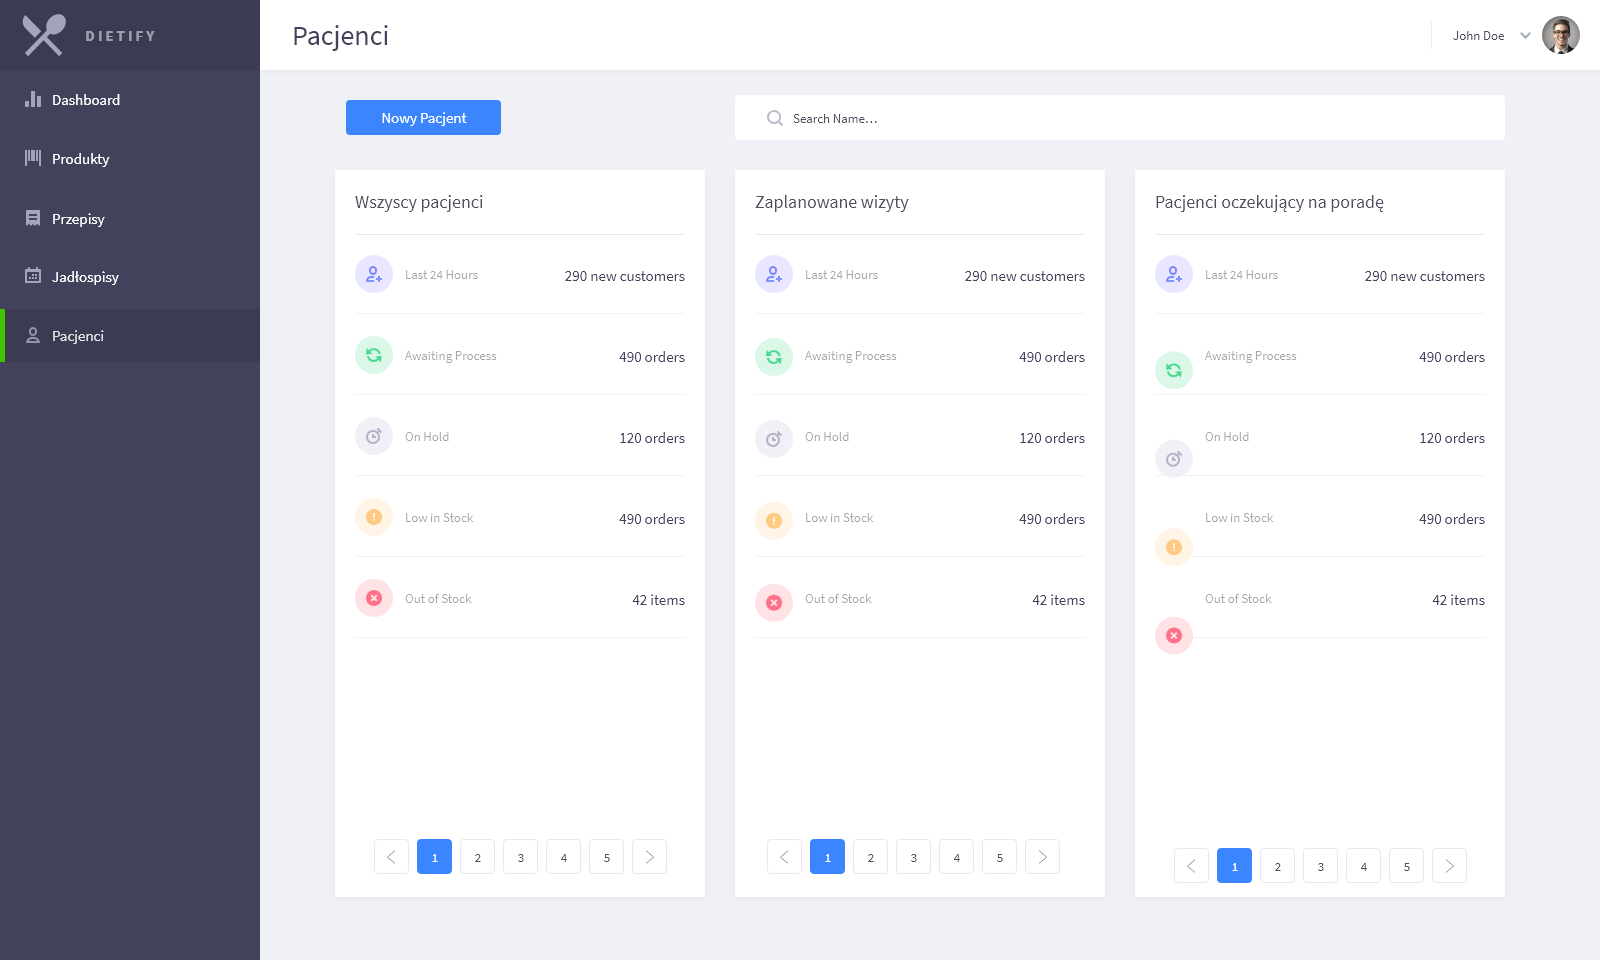
\includegraphics[width=0.9\textwidth]{img/mockups/mockup13.png}
        \caption{Mockup13 (opr.wł).}\label{rysunek:mockup13}
    \end{figure}
\end{minipage}

\begin{minipage}{\textwidth}
    \begin{figure}[H]
        \centering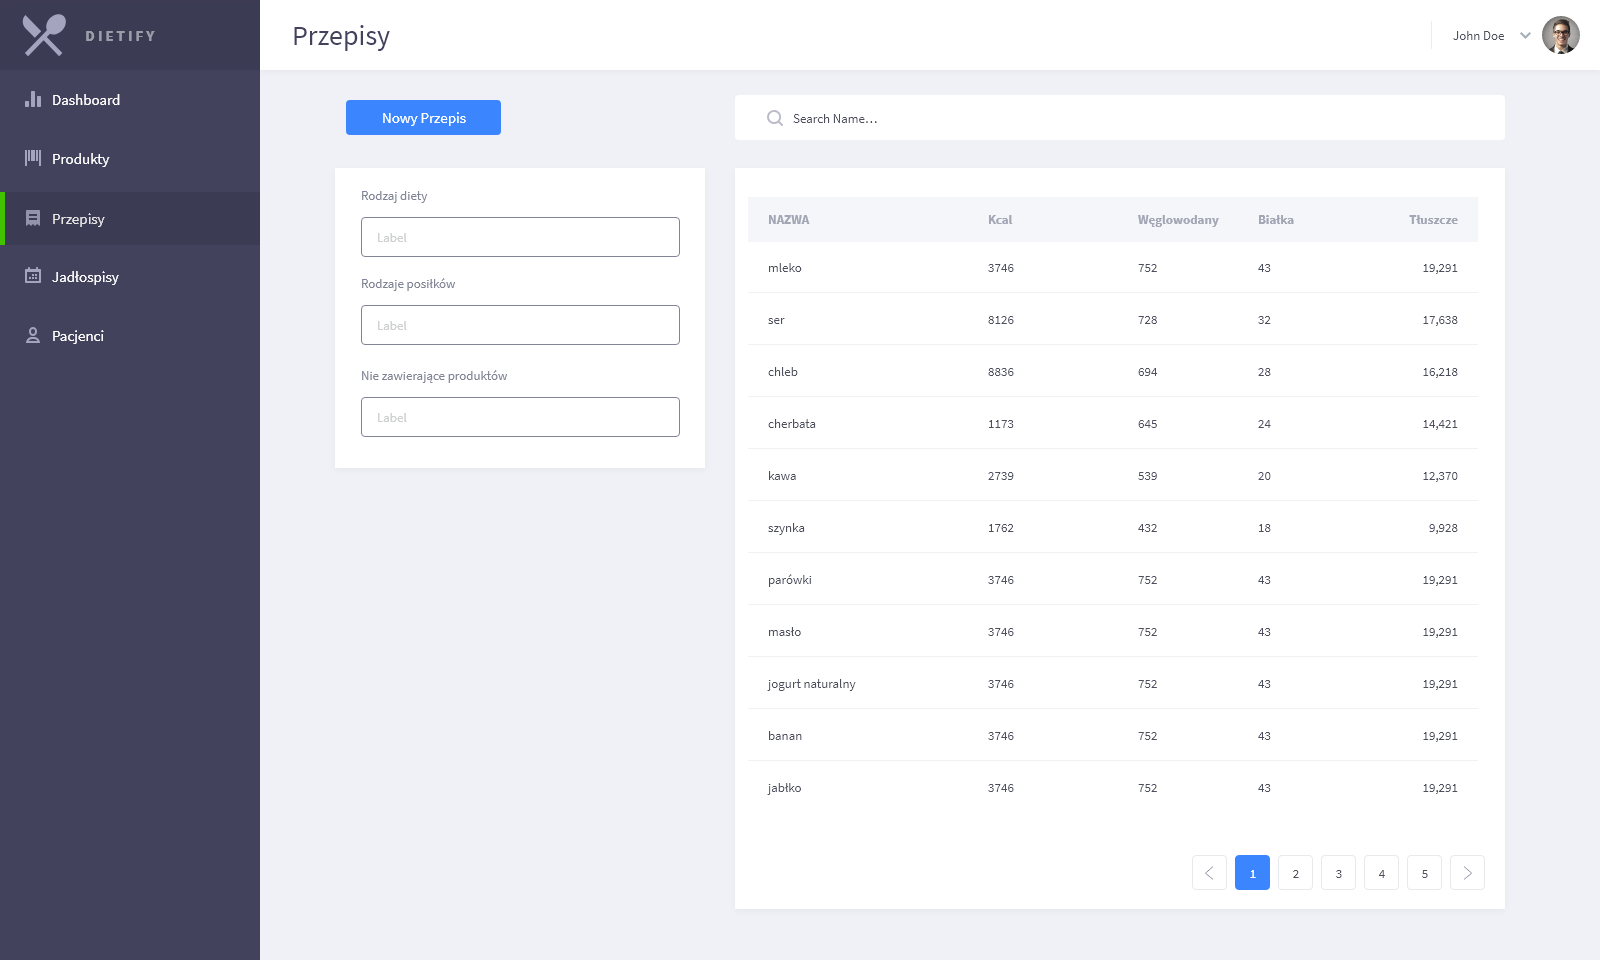
\includegraphics[width=0.9\textwidth]{img/mockups/mockup14.png}
        \caption{Mockup14 (opr.wł).}\label{rysunek:mockup14}
    \end{figure}
\end{minipage}

\begin{minipage}{\textwidth}
    \begin{figure}[H]
        \centering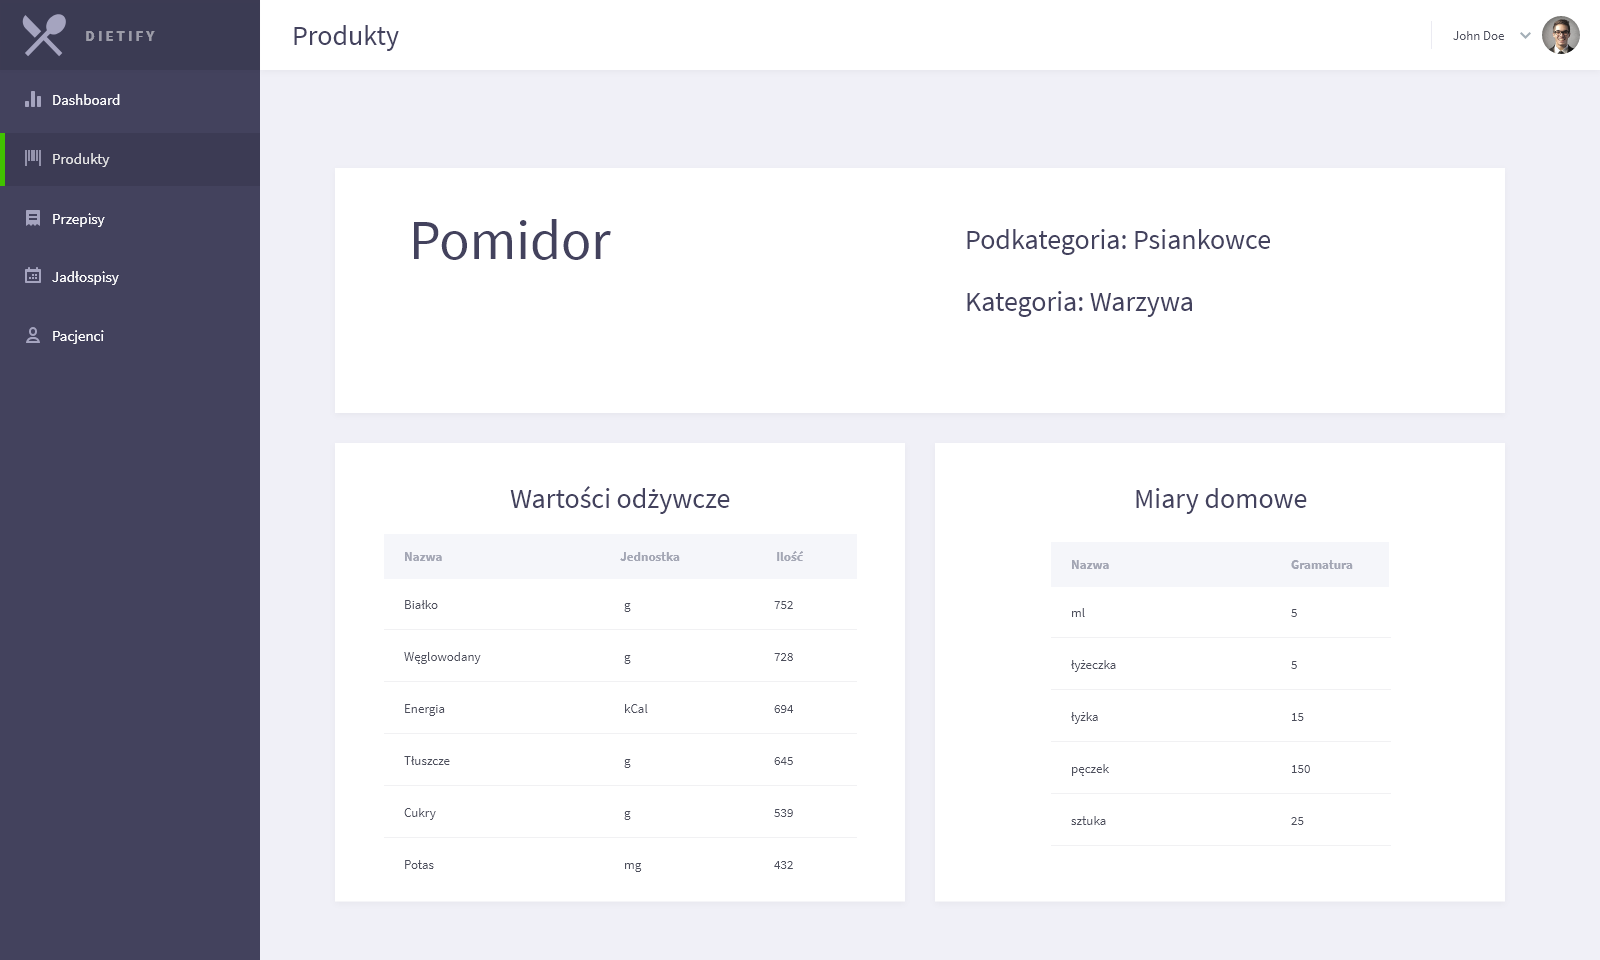
\includegraphics[width=0.9\textwidth]{img/mockups/mockup15.png}
        \caption{Mockup15 (opr.wł).}\label{rysunek:mockup15}
    \end{figure}
\end{minipage}

\begin{minipage}{\textwidth}
    \begin{figure}[H]
        \centering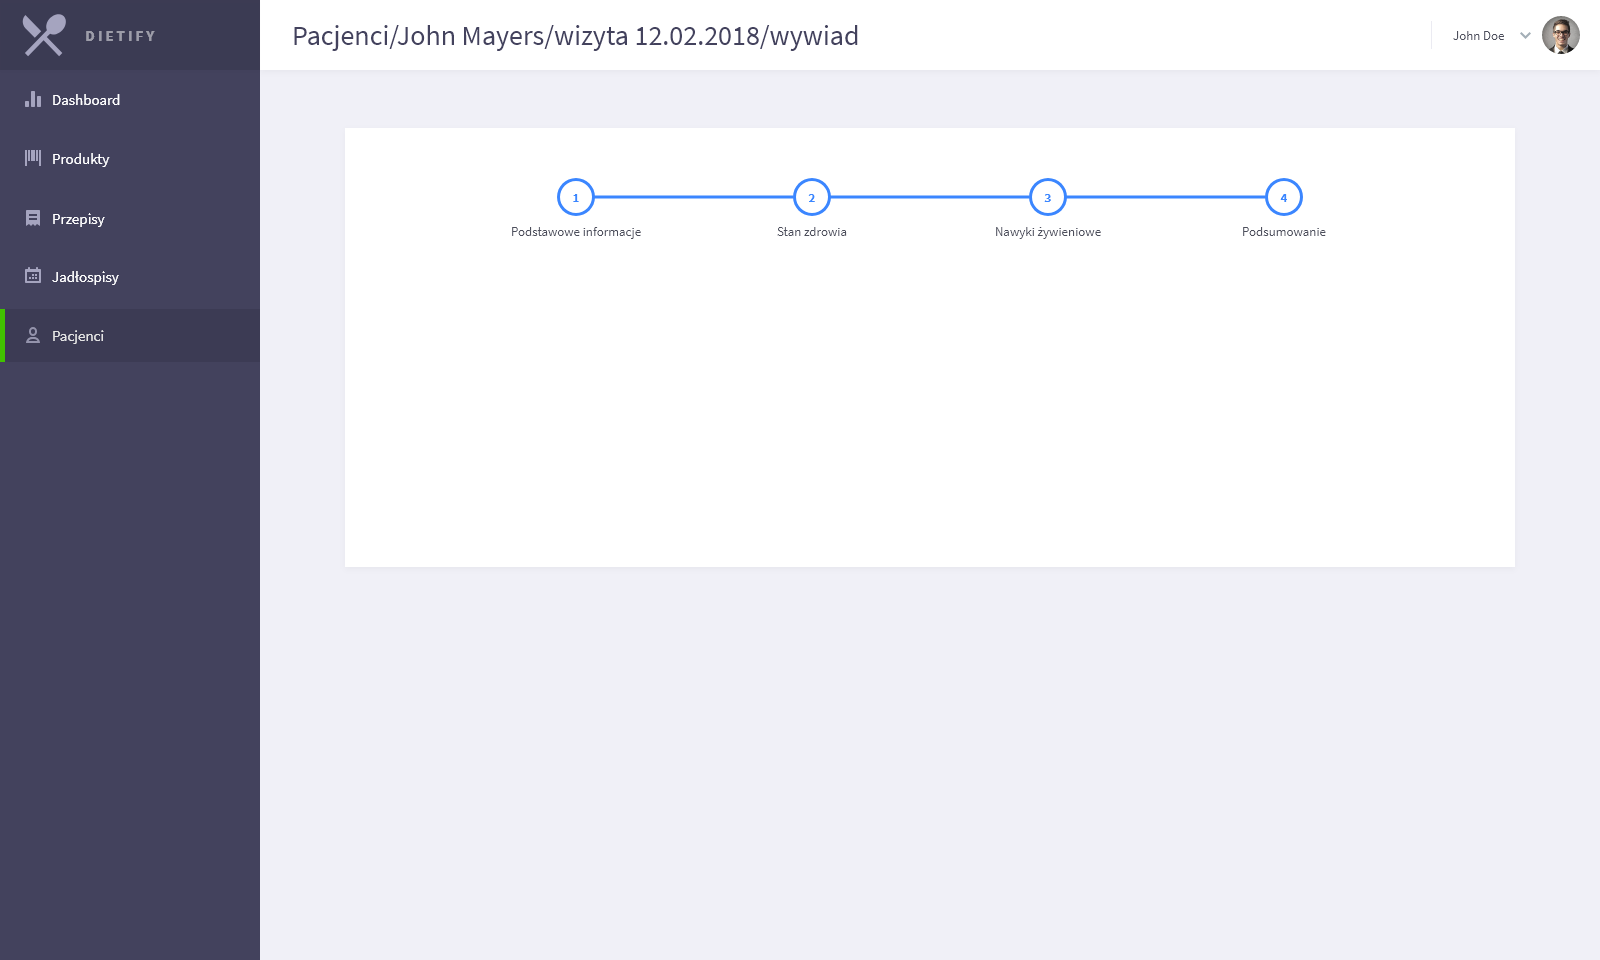
\includegraphics[width=0.9\textwidth]{img/mockups/mockup16.png}
        \caption{Mockup16 (opr.wł).}\label{rysunek:mockup16}
    \end{figure}
\end{minipage}

\section{Architektura systemu}
\subsection{Model bazy danych}

\thispagestyle{normal}
